\chapter{Introduction}
\label{ch:introduction}
Evolution is the continuous change in the heritable properties of biological communities over progressive generations. Evolutionary processes give rise to biodiversity at different levels of living organization. 
Evidence from morphological and gene sequence data suggests that all organisms on earth are genetically related, and the relationships thereof can be represented by evolutionary trees, also known as phylogenetic trees \cite{warnow2017computational}. The evolutionary history of a set of genes, species, or individuals can aid in addressing various biological inquiries. Hence, apart from being interesting on its own right, the estimation of phylogenetic trees (i.e., phylogeny estimation) is a significant step in many applications, such as, tracking the evolution of a disease, designing new drugs, investigating criminal cases, etc. \cite{bush1999predicting, aluru2005handbook}. 

Multiple sequence alignment (MSA) seeks to arrange more than two biological sequences based on certain criteria (e.g., evolutionary history, 3D structure, etc.) by inserting spaces (known as gaps) between letters in the sequences \cite{warnow2017computational}. MSA is a prerequisite subtask in several biological tasks including phylogeny estimation from sequence data, which usually comprises two phases, namely, (A) the computation of an MSA, and subsequently (B) the inference of a tree therefrom. The characteristics, as well as the quality of the MSA, obtained in Phase A dramatically influence the accuracy of the tree in Phase B. Therefore, it is important to select an MSA tool that is the “most suitable” in the phylogenetic context, suggesting the idea of (some sort of) “phylogeny-awareness” in Phase A. 

Improving the phylogeny estimation through focusing on improving MSA computation is not entirely new as is evident, albeit in a limited context, from the literature \cite{redelings2005joint, ashkenazy2018multiple, warnow2013large}. These works do suggest that the nature of MSA computation may influence the outputs (in a domain-specific manner). However, from the context of multi-objective (MO) optimization, this has not been hitherto explored. Most real-world optimization problems naturally work towards achieving several objectives. Some of these objectives are conflicting to each other. However, these problems can be transformed into single-objective ones using various simplifying techniques to avoid complexities~\citep{kalyanmoy2001multi}. On the contrary, a MO formulation defines the problem using a set of objective functions and subsequently, specialized methods can be applied to optimize all the objectives simultaneously.

In this post-genomic era, the availability and relative affordability of various sequencing technologies led to the rapid growth of biological datasets. The datasets increased in two dimensions: more species are being sequenced and longer segments of the genome are sequenced.
Hence newer datasets are posing new challenges to the researchers. Usually, an MSA method is provided with a default parameter configuration for aligning any problem instance with satisfactory accuracy. But we know that these default values can not guarantee the best output throughout all kinds of datasets~\citep{rubio2018characteristic}. For instance, there is a parameter in ProbCons called the number of iterative refinement passes. Although it can vary between 0 to 1000 the default value is set to 100. We can achieve better results by tuning the parameter values which is not a straightforward task. Moreover, despite rigorous parameter tuning, no method can consistently outperform other methods for all datasets. 

As no single objective is biologically guaranteed to lead to the most accurate solution, identifying a set of MSA objectives that are more useful in the context of Phylogeny estimation, i.e., phylogeny-aware objectives, seems appealing. But, here we are confronted with the arduous challenge of choosing suitable measures/metrics to optimize from among a variety of objective functions- new or from among the ones available in the literature. So, we ask the obvious question of whether the generic metrics, widely used for assessing the alignment quality, will accurately represent the level of acceptance in the context of a specific application domain, i.e., in our case, phylogeny estimation. This question has indeed received some discussions, albeit shallow and incomplete, in several studies (\cite{mirarab2015pasta, liu2009rapid}). However, we are not aware of any systematic investigation in the literature to this end.

There are different categories of MSA methods available in the literature. We can broadly divide them into three groups: progressive techniques, consistency-based techniques, and iterative techniques. This division is not exclusive as many tools also use a combination of these techniques. The progressive methods (e.g., Clustal $\Omega$~\citep{sievers2011fast}, FSA~\citep{bradley2009fast}) compute the alignment using a guide tree by aligning pairs of sequences in a ``bottom-up'' manner. The consistency-based techniques (e.g., T-Coffee~\citep{notredame2000t}, ProbCons~\citep{do2005probcons}) first construct a database of local and global pairwise alignments to facilitate generating an overall accurate alignment. 
And the most flexible methods are the iterative methods (e.g., SATe-II \cite{liu2012sate}, PASTA \cite{mirarab2015pasta}). These are particularly appealing because of their ability to fix errors made in the earlier stages of computation by repeating some steps until an optimization criterion or objective function, quantifying the quality of the (re)alignment, converges. Once the challenging task of identifying phylogeny-aware objectives is successful a natural idea would be to incorporate those in these celebrated tools and conduct a comparative study among those.    

Another related and complicated problem arises when inferring phylogeny from genome-wide data comprising longer sequences. In such a scenario, the evolutionary histories can change across different parts of the genome due to biological processes known as incomplete lineage sorting, gene duplication and loss, etc. This has led to the development of new phylogenomic methods at the intersection of phylogenetics and genomics. In this context, the evolutionary relationships of a group of organisms is called the species tree. On the other hand, the phylogeny specific to a particular region of the genome (known as locus or gene) is termed as a gene tree \cite{maddison1997gene}. Incomplete lineage sorting (ILS), modeled by the multi-species coalescent (MSC), is considered to be a dominant cause for gene tree incongruence \cite{mirarab2014evaluating, statistical-binning}. Various optimization criteria (e.g., quartet score, pseudo-likelihood, etc.) are statistically consistent under the MSC model, meaning that they return the true species tree with high probability given sufficiently large numbers of accurate gene trees. However, the number of genes is limited and estimating highly accurate gene trees is difficult. Therefore, even popular methods, optimizing a particular criterion, may fail to reconstruct highly accurate trees under practical model conditions with limited numbers of genes and in the presence of gene tree estimation error. In this context as well, the MO optimization framework seems appealing with phylogeny-aware objective functions.

\section{Research Gap}
In this thesis we carefully examine the existing studies on phylogenetic analyses and identify the following research gaps which will be further discussed in the subsequent chapters.
\begin{enumerate}
	\item  More research effort need to be employed to combine the strength of different approaches in a generic way to tackle the challenges of the post-genomic era as no single method can provide high accuracy across different data. 
	
	
	\item  General purpose MSA performance measures which are currently widely-used in the literature may not be adequate to reflect the actual purpose of MSA such as phylogeny estimation, protein structure prediction, etc.
	
	
	\item  Lack of systematic study to leverage multiple MSA objectives from different studies for better phylogeny estimation over a broad range of data.
	
	
	\item  No solid theoretical/empirical ground in the literature for choosing the appropriate objective functions from numerous existing objectives  or newly proposed.
	
	
	\item No systematic endeavor effort found in the literature to improve the performance of summary methods for species tree estimation by combining multiple statistically consistent criteria.
\end{enumerate}

To address all these research gaps mentioned above, we \textbf{TBD}
A high-level

\begin{figure}[!htbp]
	\centering
.	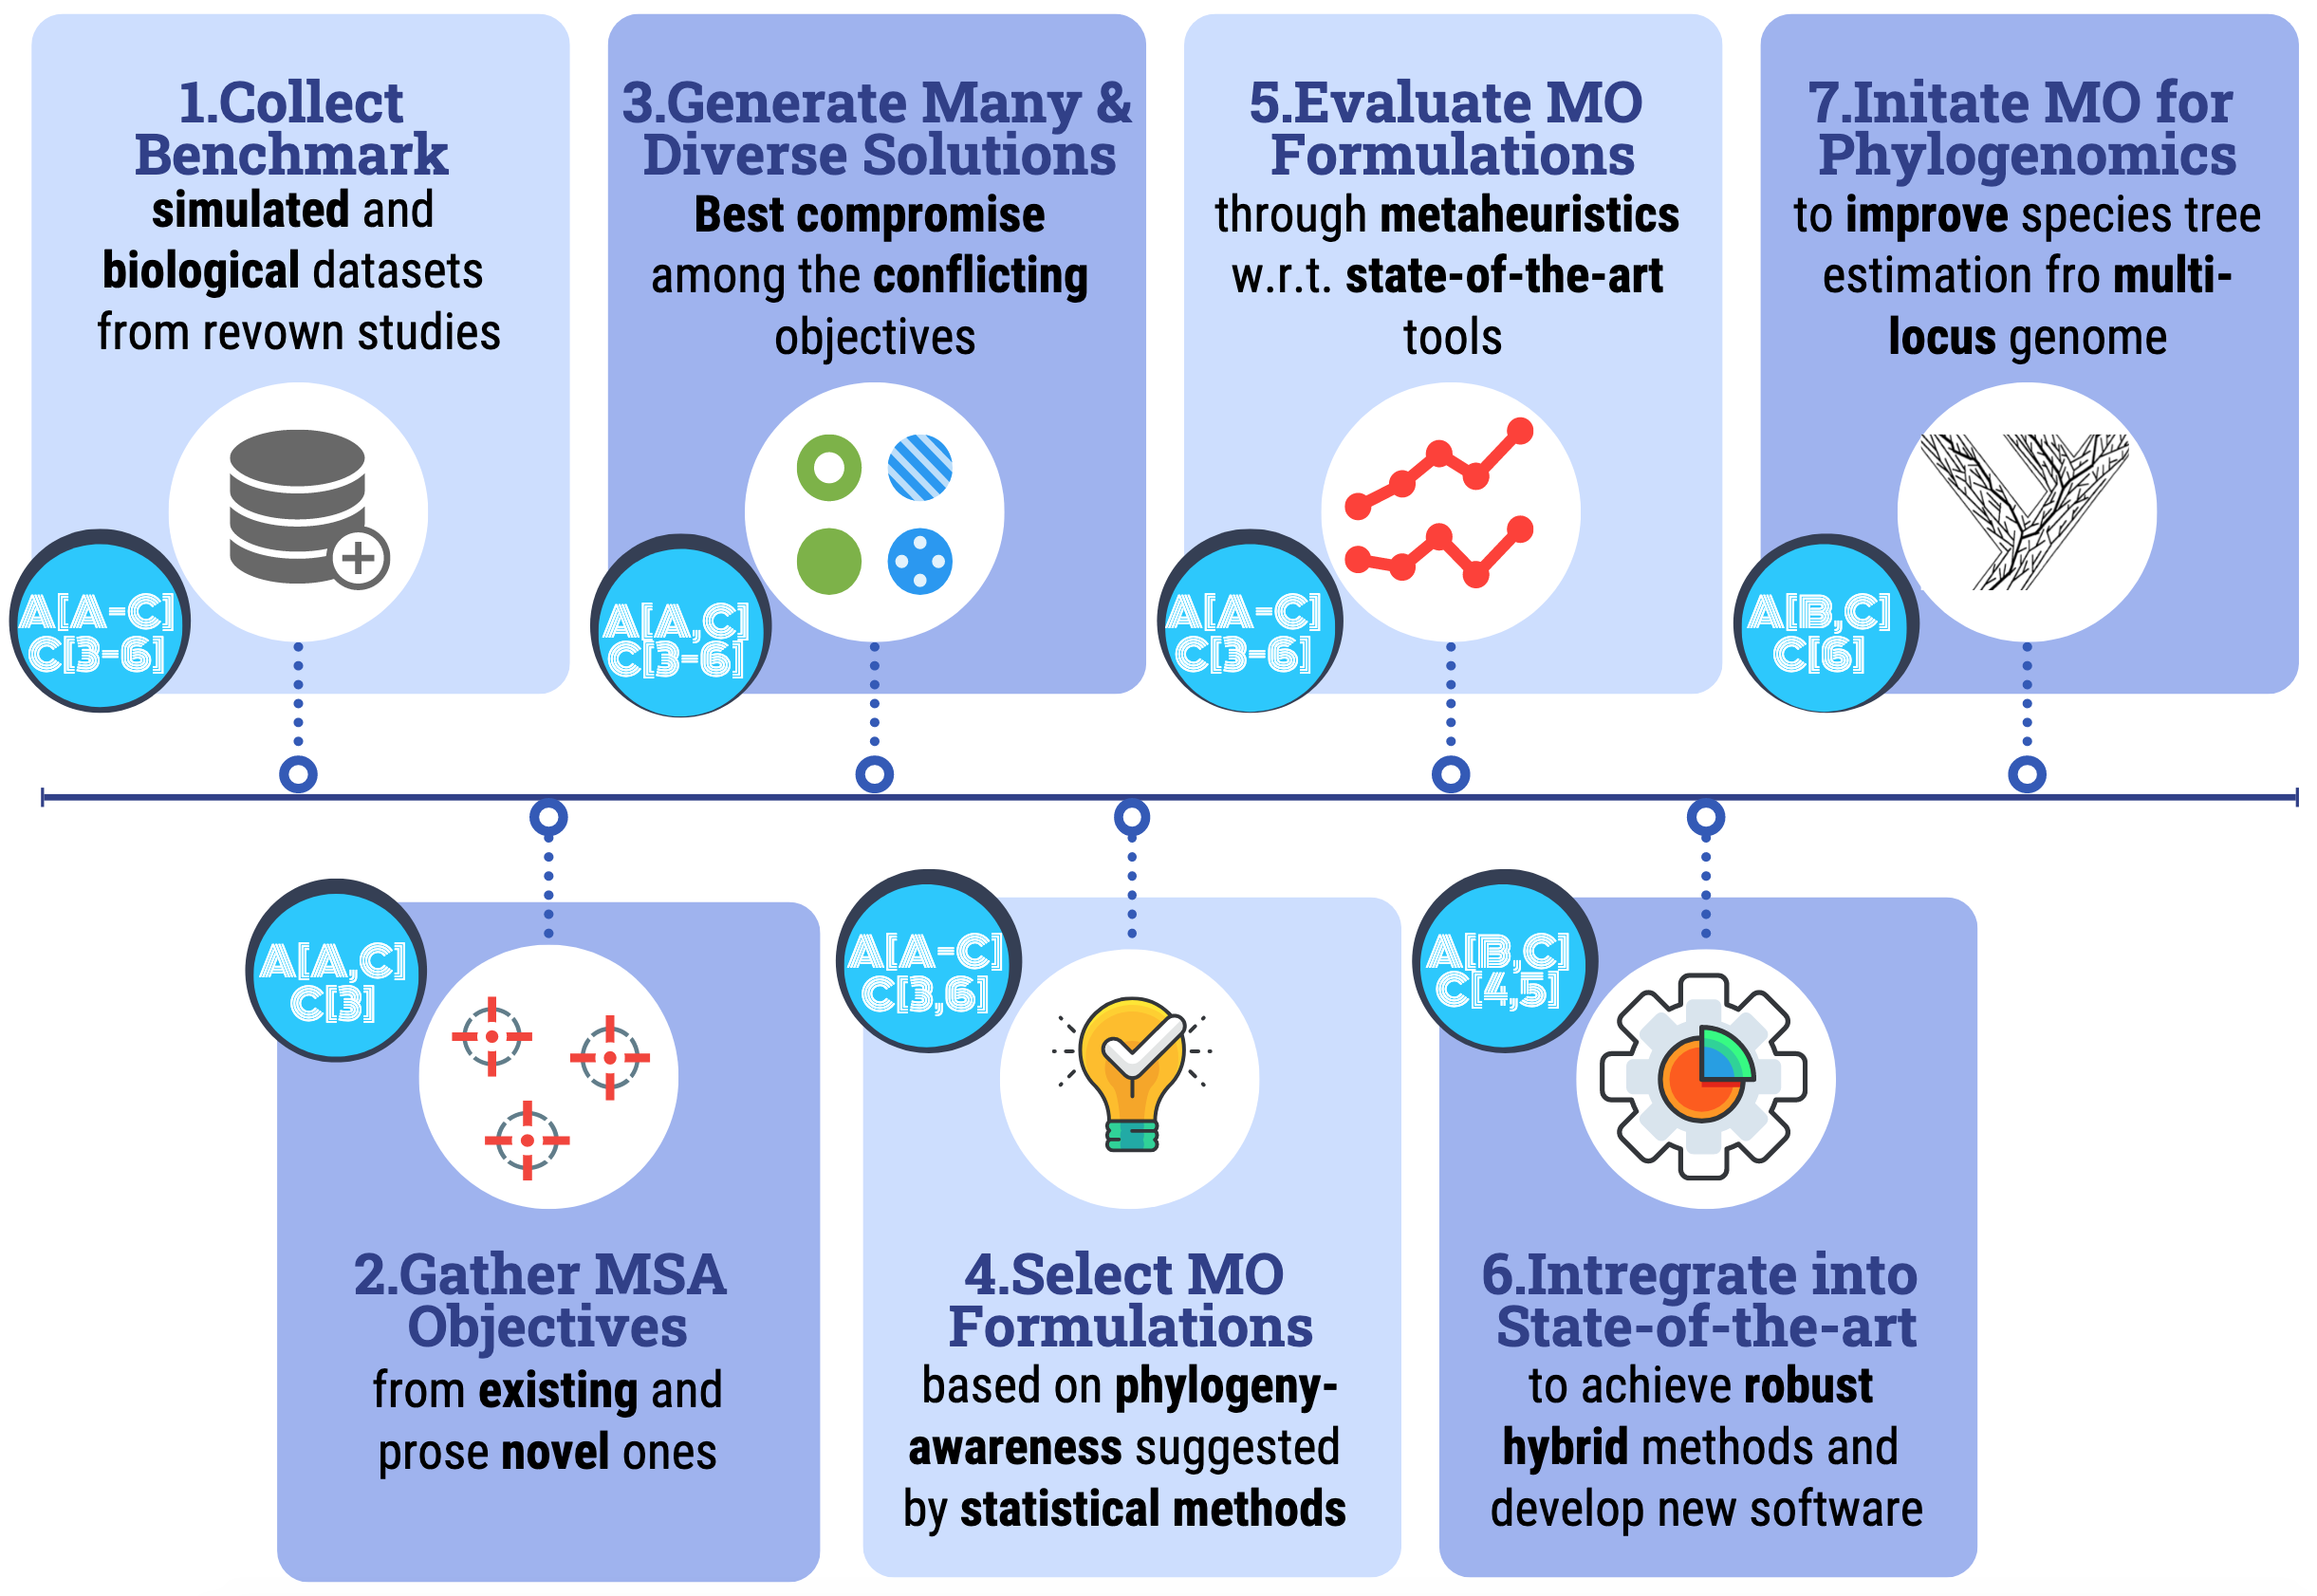
\includegraphics[width=1.0\textwidth]{Figure/research-overview-new}
	\caption[A high-level overview of the research works conducted in this thesis]{A high-level overview of the research works conducted in this thesis. Each box depicts a research components which is mapped to our overarching aims denoted by $A[x,y,...]$ and chapters denoted by $C[x,y,...]$ inside a blue circle embedded within the box.
		Research component 1: we collect simulated and biological datasets to conduct our experiments from renowned studies.
		Research component 2: we study and short-list several objective functions widely used in the literature as well as some novel ones to compute MSA based on their efficacy.
		Research component 3: We adapt popular MO metaheuristics which simultaneously optimize several objectives to generate a large collection of diverse solutions that represent the best compromise among the conflicting objectives. For each alignment we generate a phylogenetic tree using a standard approach.
		Research component 4: We select some MO formulations of MSA and related problems based on their observed association with a phylogeny-aware measure through rigorous statistical methods.
		Step 5: We run selected  MO metaheuristics on the selected formations and compare the generated alignments and trees to that of the state-of-the-art tools.
		Research component 6: We incorporate all the phylogeny-aware objectives within state-of-the-art MSA methods with a goal to improve their robustness through MO strategy.
		Research component 7: We formulate the task of species tree estimation by summarizing a set of discordant gene trees as MO optimization task by accumulating the optimization criterion of the state-of-the-art summary methods.}
	
	\label{fig:research-workflow}
	
\end{figure}

\section{Thesis Objectives}

To address the research gaps mentioned earlier, our overarching goal is three-fold as follows. Firstly, we aim to investigate whether a domain-specific measure is useful in MSA computation and develop a systematic methodology to leverage such a measure (Aim A). Secondly, we want to advance the state of the art of phylogeny estimation and closely related problems like species tree estimations (Aim B), and thirdly, we want to achieve this advancement through leveraging the multi-objective optimization framework (Aim C). In our case, the domain principally is phylogeny estimation and hence we introduce the concept of ‘phylogeny-awareness’. A research workflow diagram for this thesis is shown in Figure~\ref{fig:research-workflow}. Below, we mention the direct relation to the aims above in square brackets. The main objectives of this thesis are as follows:

\begin{enumerate}
\item To systematically investigate whether the generic metrics, widely used for assessing the alignment quality, can accurately represent the level of acceptance in the context of a specific application domain, i.e., in our case, phylogeny estimation. And in this context, to investigate, how useful the phylogeny-aware objectives are. [Aim A]

\item To develop a systematic methodology to select phylogeny-aware multi-objective formulations of MSA. [Aim A, C]

\item To adapt state-of-the-art multi-objective optimization algorithms/frameworks to tackle our obtained phylogeny-aware multi-objective formulations of MSA. [Aim A-C]

\item To develop customized multi-objective algorithms to infer species trees by summarizing a set of given gene trees. [Aim B, C]

\item To incorporate many phylogeny-aware objective functions into the workflow of several state-of-the-art iterative MSA tools. [Aim A, C]

\item To develop a user-friendly software tool that helps researchers to estimate phylogenetic trees from MSAs using our proposed approaches. [Aim B]
\end{enumerate}

\section{Our Contribution}
This thesis addressed some notable challenges in computing high-quality phylogenetic trees from sequence alignments and thereby made the following contributions.

\subsection{Systematic method to detect appropriate MO formulations}
 We developed a systematic methodology for choosing an appropriate multi-objective formulation of MSA considering the application domain with the help of rigorous statistical methods like multi-variate linear regression. We considered phylogeny estimation to be the intended application of MSA in this thesis,.

\subsection{Phylogeny-aware MO formulations}
 We proposed several phylogeny-aware multi-objective formulations of MSA considering their high potential to yield better phylogenetic trees. We experimental demonstrated that these formulations can yield better solutions compared to the existing methods.

\subsection{Hybridization of state of the art and MO principles}
 We developed some robust methods for alignment-based phylogeny estimation stemming from the hybridization of state-of-the-art iterative MSA methods and many-objective optimization strategies by carefully embedding several phylogeny-aware objective functions within the workflow of those MSA methods. 

\subsection{Custom MO phylogenomic approach to infer species tree}
 We designed some customized multi-objective optimization algorithms for genome-wide species tree estimation by summarizing a set of heterogeneous gene trees. The proposed algorithms could be of independent interest to the multi-objective optimization research community.

\subsection{Open Source flexible software framework}
 We developed an Open Source software framework for estimating phylogenetic trees from MSAs using our proposed approaches. Its components can potentially be modified, replaced or further refined by bioinformatics researchers and practitioners.

\subsection{Comparative study}
 We presented a scientific discourse along with a comparative analysis on the overall efficacy of the concept of domain-specific measures in general and phylogeny-awareness in particular. It could be useful in a generic way in any branch of science and engineering.



\section{Thesis Organization}

The rest of the thesis is organized as follows.

In Chapter~\ref{ch:background} we introduce preliminary concepts and terminologies of computational phylogenetics
relevant to the contribution of this thesis. We introduce the optimization task of phylogeny estimation and MSA computation. We present different methodologies and metrics to evaluate the performance of that task. Since we employ multi-objective optimization strategies in this thesis, we, therefore, discuss its basic concepts along with some popular multi-objective metaheuristics.

Chapter~\ref{ch:cybernatics} begins with a discussion on the present state of the MSA methods. Afterward, we gradually develop a systematic methodology for choosing an appropriate multi-objective formulation of MSA considering the application domain (i.e., in our case phylogeny estimation). With the help of state-of-the-art multi-objective metaheuristics and Rigorous statistical methods like Multi-variate linear regression, we identify two phylogeny-aware bi-objective formulations of MSA. Then we evaluate the performance of the phylogeny-aware formulations compared to the state-of-the-art single objective MSA methods. Thereby we present a scientific discourse along with a comparative analysis on the overall efficacy of the concept of domain-specific measures in general and phylogeny-awareness in particular. 

In Chapter~\ref{ch:pmao}, we exploit our findings from Chapter~\ref{ch:cybernatics} by designing the PMAO framework, based on PASTA which is one of the most celebrated MSA tools. Here we incorporate many phylogeny-aware objective functions within PASTA through principles of multi-objective optimization, to generate a bunch of high-quality phylogenetic trees. We innovatively employ supervised machine learning within the PMAO framework to generate a smaller number of top solutions to assist the domain expert in choosing the final solution through visual inspection. We experiment with summarizing the PMAO outputs using greedy consensus and quartet consistency to obtain a single high-quality solution without using any external evidence.

%a robust method for alignment-based phylogeny estimation stemming from the hybridization of many-objective optimization strategies and PASTA which is one of the most celebrated MSA tools.

In Chapter~\ref{ch:mammle}, we introduce MAMMLE, a framework for inferring better phylogenetic trees from unaligned sequences by hybridizing MUSCLE with a multi-objective optimization strategy and leveraging multiple Maximum Likelihood hypotheses. MAMMLE is a flexible framework whose components can potentially be modified, replaced, or further refined by bioinformatics researchers and practitioners. We provide the Linux and Mac OS X implementation of MAMMLE as an Open Source tool.
%we present an Open-source software for estimating phylogenetic trees from MSAs using our proposed approaches. 


Chapter~\ref{ch:snoga} focuses on species tree estimation from multi-locus data. Here we explicitly consider that different regions within the genome can evolve independently and the species tree should be reconstructed as a generalization of the gene lineages. After discussing the present state of the problem, we formulate the task as a multi-objective task utilizing different statistically consistent criteria from existing summary methods and design a customized multi-objective optimization algorithm.


Finally, we conclude our thesis by summarizing the major contributions and findings, outlining future directions for extending the accomplished research works, and discussing some of our ongoing works inspired by the central theme of this thesis in Chapter~\ref{ch:conclusion}.

\begin{comment}

By accomplishing our objectives mentioned above we expect to obtain the following outcomes.
%The possible outcomes of this research are as follows:

(i) A systematic methodology for choosing an appropriate multi-objective formulation of MSA considering the application domain (i.e., in our case phylogeny estimation). [Aim A, C]

(ii) Several phylogeny-aware multi-objective formulations of MSA. [Aim A, C]

(iii) Some robust methods for alignment-based phylogeny estimation stemming from the hybridization of state-of-the-art iterative MSA methods and many-objective optimization strategies. [Aim A-C]

(iv) Some customized multi-objective optimization algorithms for species tree estimation by summarizing a set of given gene trees. [Aim B, C]

(v) As a by-product of the above outcome, new MO frameworks may be proposed that could be of independent interest. [Aim C]

(vi) Open-source software tools for estimating phylogenetic trees from MSAs using our proposed approaches. [Aim B]

(vii) A scientific discourse along with a comparative analysis on the overall efficacy of the concept of domain-specific measures in general and phylogeny-awareness in particular. [Aim A]
\end{comment}